% Generated by thesis/ch7/exp2/networks.py -- do not edit by hand.
\begin{sidewaysfigure}
  \centering
  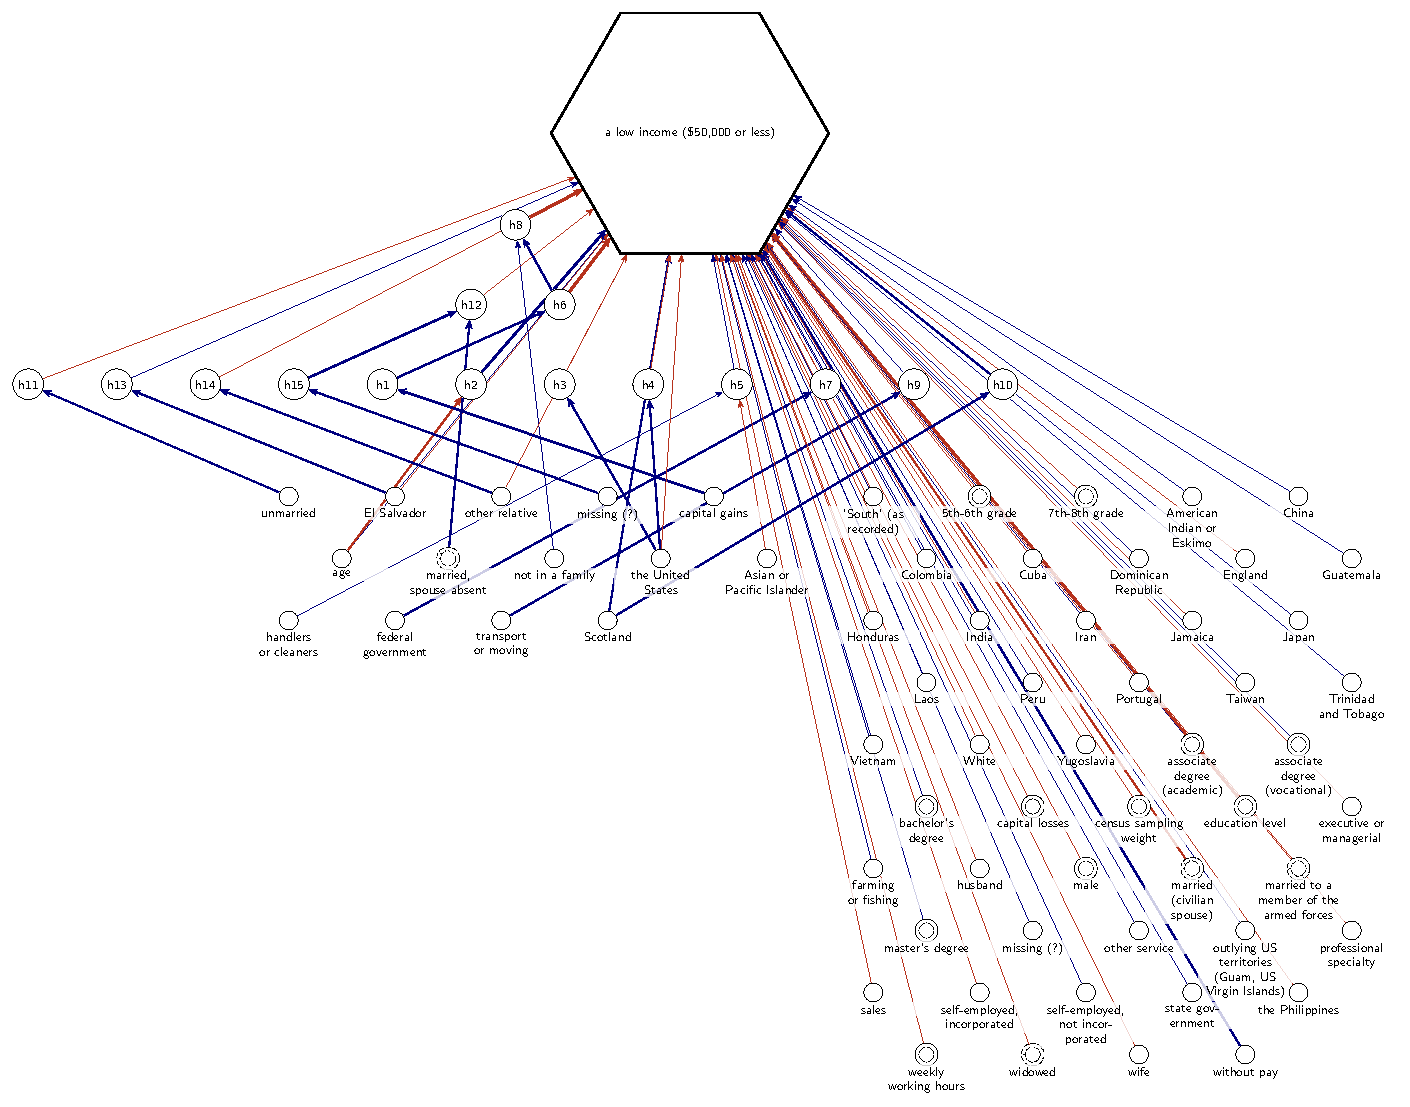
\includegraphics[width=\textheight,height=0.78\textwidth,keepaspectratio]{figures/exp2/networks/adult-s3-raw}
  \caption{Adult, seed 3 (adult-s3): the network as trained, before any explanation, in full. Inputs at the bottom (every input column its own node), hidden units by depth, the output at the top; 63 of 107 input columns are connected, with 15 hidden units and 85 enabled connections. Blue: positive weight (raises the score); red: negative weight (lowers it); thicker: larger weight. Orange outline and up arrow: raises the final prediction; teal and down arrow: lowers it; grey and double arrow: depends. Not used (no connection; 44 columns): missing (?), local government, never worked, private, 10th grade, 11th grade, doctorate, high-school graduate, preschool, professional school degree, some college, 12th grade (no diploma), 1st-4th grade, 9th grade, divorced, never married, separated, administrative or clerical, protective service, technical support, armed forces, craft or repair, machine operator or inspector, private household service, own child, Black, other race, Cambodia, France, Germany, Greece, Haiti, the Netherlands, Hong Kong, Hungary, Canada, Ireland, Italy, Mexico, Nicaragua, Poland, Puerto Rico, Thailand and Ecuador.}
  \label{fig:exp2-net-adult-s3-raw}
\end{sidewaysfigure}
